% Data figure, generated by export_eab3.py (third round; panel (b) audits development) (figures/fig-evidence.pdf).
\begin{figure*}[t]
\centering
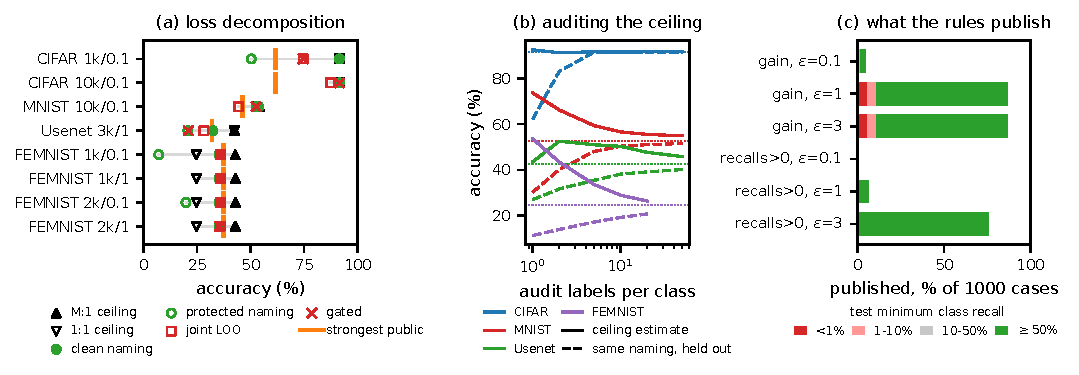
\includegraphics[width=\textwidth]{figures/fig-evidence.pdf}
\Description{Loss decomposition per task, audit-sample ceiling estimates
versus held-out naming accuracy, and the minimum test class recall of
published classifiers.}
\caption{(a) Table~\ref{tab:decomposition} as a decomposition: each row
moves from the partition ceilings to noise-free naming (teacher content),
protected naming (release noise) and selected classifiers (selection);
the vertical bar is the strongest public learner. (b) A random labelled
audit of the development split: its in-sample one-to-one ceiling estimate
(solid) and the test accuracy of the naming it induces (dashed); dotted lines
are the true ceilings; 200 repetitions. (c) The 1000 cases per budget of
Table~\ref{tab:verify-ladder}, by the test minimum class recall of the
classifier each rule publishes. All panels are offline diagnostics.}
\label{fig:evidence}
\end{figure*}
